\section{Eletromiografia de Superfície (sEMG)}

A eletromiografia consiste em uma técnica de registro da atividade elétrica produzida pelos músculos esqueléticos durante a contração. Quando um neurônio motor dispara, propaga-se ao longo das fibras musculares uma diferença de potencial denominada potencial de ação da unidade motora (PAUM). A eletromiografia de superfície (sEMG) capta a superposição temporal e espacial desses PAUMs por meio de eletrodos posicionados sobre a pele, de forma não invasiva, diferindo da eletromiografia intramuscular, que utiliza agulhas inseridas diretamente no tecido muscular.\cite{Costa}
\begin{figure}[htbp]
    \centering
    \caption{Ilustração do processo de aquisição de sinais sEMG}
    \label{fig:ilustracaosensor}
    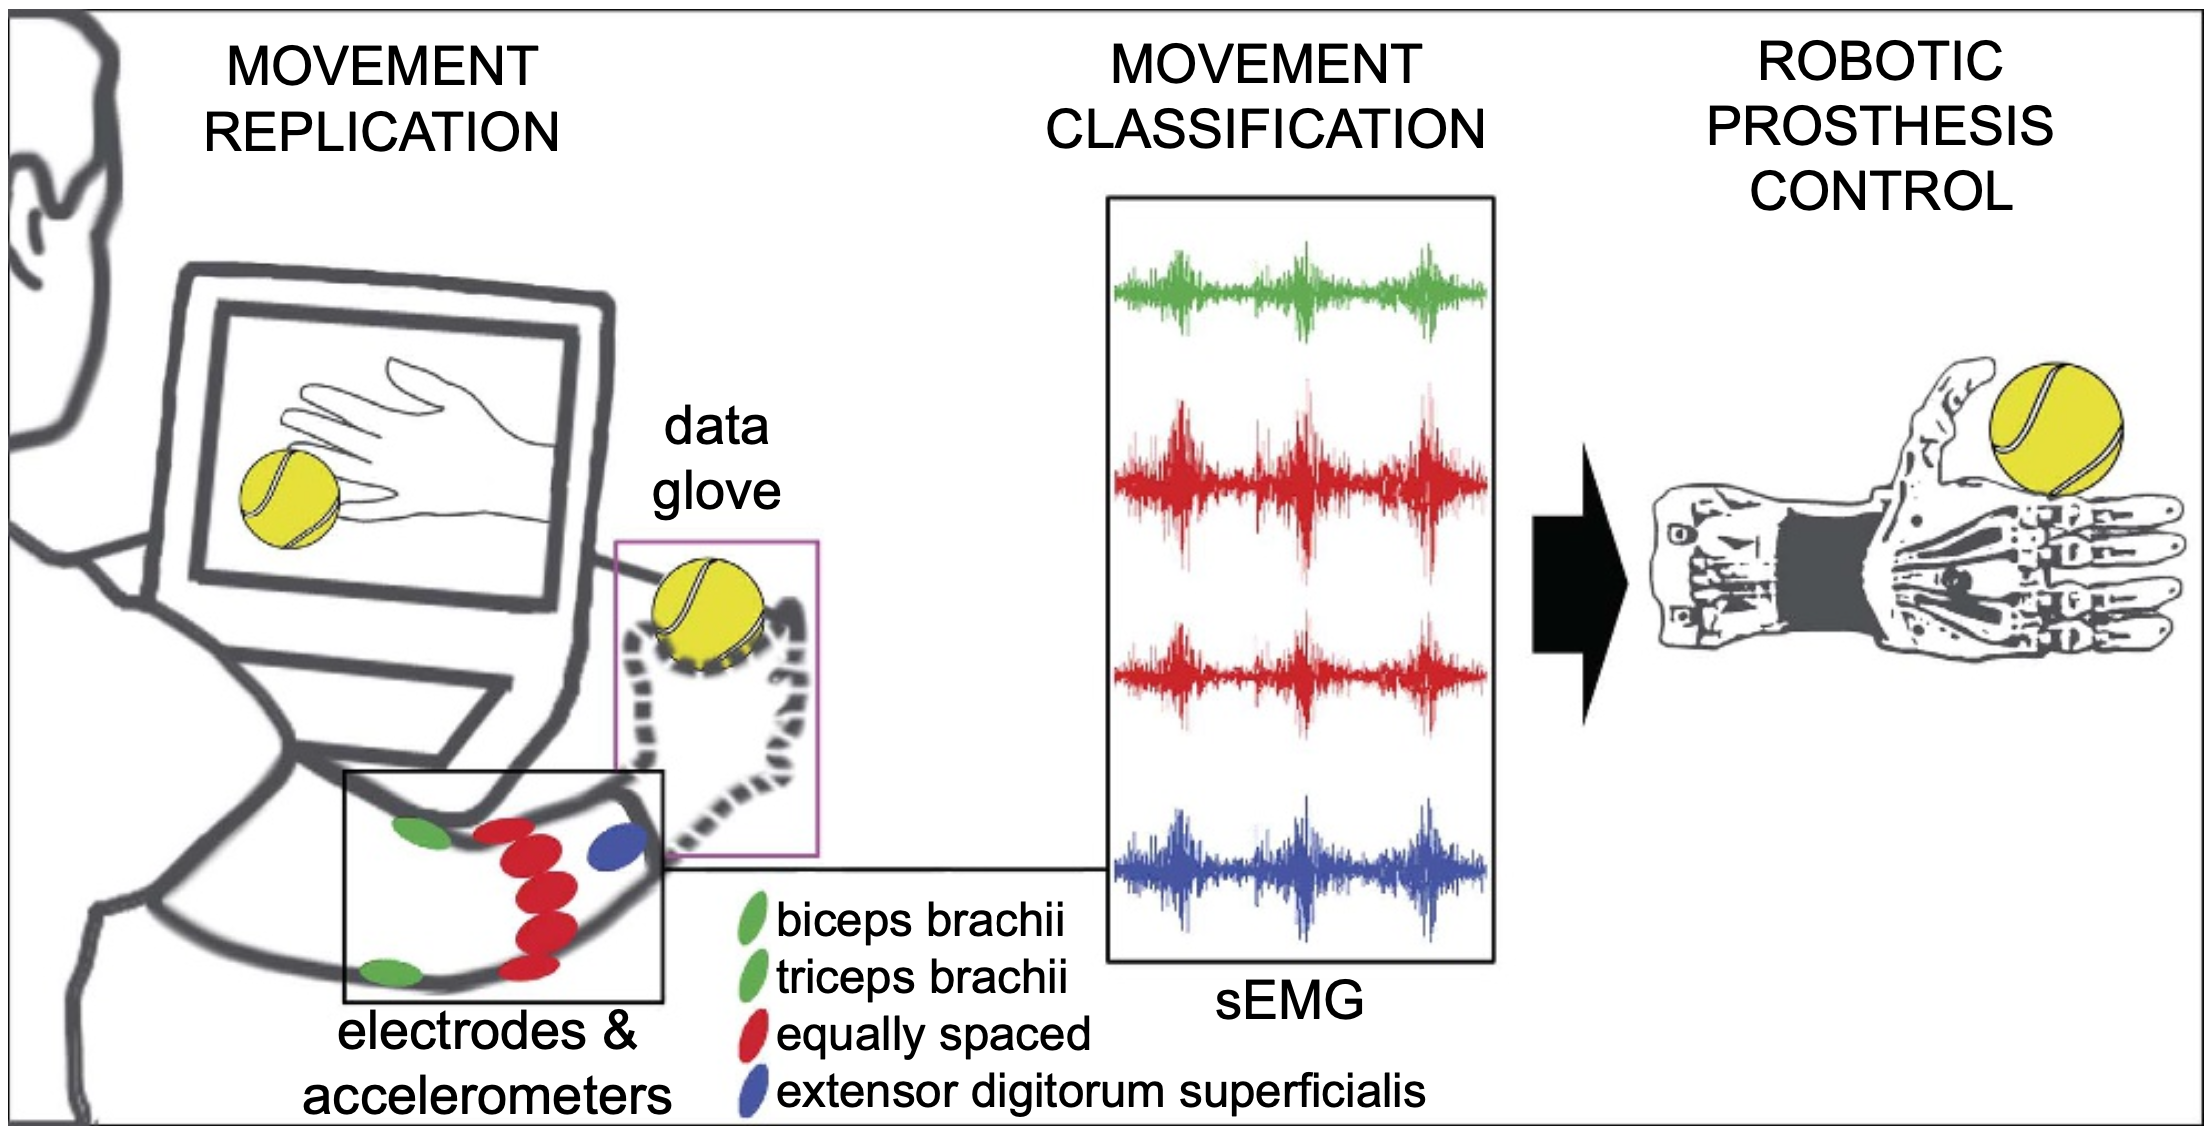
\includegraphics[width=0.8\textwidth]{2_fundamento_teorico/assets/SData_Protocol.png}
    \fonte{\cite{Ninapro}.}
\end{figure}

O sinal sEMG apresenta amplitude tipicamente entre 1 mV e 10 mV, frequências úteis na faixa de 20 Hz a 500 Hz, elevada sensibilidade a ruídos e forte dependência de fatores como posicionamento dos eletrodos, espessura do tecido subcutâneo, temperatura e fadiga muscular. Suas principais fontes de interferência incluem o ruído da rede elétrica (50/60 Hz), artefatos de movimento dos eletrodos, ruído térmico (Johnson), crosstalk de grupos musculares adjacentes e artefatos de movimento corporal.
Para minimizar essas interferências, é necessário um cuidadoso condicionamento do sinal, composto tipicamente por um amplificador de instrumentação (ganhos entre 100 e 1000), filtros passa-altas (corte em torno de 20 Hz para remoção de artefatos DC e de movimento), filtros passa-baixas (corte em 500 Hz), filtro notch (50 ou 60 Hz) e, opcionalmente, etapas de retificação e extração de envoltória para análise de amplitude.\cite{CLANCY20021}
